\documentclass[11pt]{article}
\usepackage[a4paper,margin=2.5cm]{geometry}
\usepackage[T1]{fontenc}
\usepackage[utf8]{inputenc}
\usepackage{amsmath,amssymb}
\usepackage{booktabs,array}
\usepackage{graphicx}
\usepackage{xcolor}
\usepackage[numbers,sort&compress]{natbib}
\usepackage[colorlinks=true,linkcolor=blue!50!black,citecolor=blue!50!black,urlcolor=blue!50!black]{hyperref}

\newcommand{\q}[1]{qg_{#1}}
\newcommand{\qZ}{qg_Z}
\newcommand{\qX}{qg_X}
\newcommand{\qY}{qg_Y}

\title{El radio de Bloch local como lectura de entrelazamiento:\\
qué restituye el filtro de simetría qg y qué no}
\author{Vicente Humberto Monteverde\\
\small Universidad del Museo Social Argentino (UMSA), Argentina\\
\small ORCID 0000-0001-8884-4811}
\date{\small Borrador del 4 de octubre de 2026}

\renewcommand{\abstractname}{Resumen}
\renewcommand{\tablename}{Tabla}
\renewcommand{\figurename}{Figura}
\renewcommand{\refname}{Referencias}

\begin{document}
\sloppy
\maketitle

\begin{abstract}
Los valores qg locales de cada qubit, $(\qX,\qY,\qZ)$, son un punto de la bola de Bloch. Su distancia al centro al
cuadrado, $r^2=\qX^2+\qY^2+\qZ^2=2\,\mathrm{Tr}\rho_q^2-1$, es el radio de la esfera sobre la que vive el qubit (área
$4\pi r^2$). Si el registro es puro, el déficit $1-r^2$ es el entrelazamiento conocido del qubit con el resto
(one-tangle); con ruido mezcla entrelazamiento e impureza. Mostramos que los circuitos que conservan el peso de Hamming
eliminan esa ambigüedad bajo un modelo de ruido. En un estado de peso fijo $\qX=\qY=0$ en todos los qubits, así que
$r=|\qZ|$ y el déficit se lee solo con disparos en la base Z; con amortiguamiento igual en todos los qubits, el filtro
de simetría qg devuelve exactamente el estado sin ruido, y el déficit filtrado es el entrelazamiento sin ruido. En una
simulación pre-registrada (90 configuraciones) coincide con él a $3\times10^{-15}$ y en estados producto es exactamente
cero, mientras que sin filtro aparece un déficit falso de 0.60--0.95. En cinco modelos de ruido de equipos (tres de IBM,
dos de IonQ) el filtro reduce entre 3.2 y 4.0 veces el error del déficit en circuitos entrenados, pero quita solo entre
el 15 y el 33\,\% del déficit falso de un estado producto: los errores que mueven una excitación dentro del sector pasan
el filtro, y cerca de un polo el déficit los amplifica como $4\varepsilon(1-\varepsilon)$. El radio también separa el
ángulo polar en radianes de la longitud del vector, $\theta=\arccos(\qZ/r)$: este ángulo es exacto con ruido
despolarizante, donde $\arccos\qZ$ se equivoca hasta 0.7 rad, y es entre 5 y 9 veces más preciso en los modelos de
ruido de equipos cuando las compuertas de ruido se ejecutan de verdad. Tres de diecinueve predicciones fallaron y se
informan. Todo se reproduce con la librería abierta \texttt{qang} (versión 0.6.8, \texttt{pip install
qang}).
\end{abstract}

\section{La pregunta}

El proyecto qang describe un qubit con cantidades de medición, el sesgo polar $\qZ=\langle\sigma_z\rangle$ y sus
compañeros~\cite{monteverde2026qang}. Un agregado natural, propuesto en este proyecto, es la esfera sobre la que vive
cada qubit: su radio $r$, o lo que es lo mismo su área $4\pi r^2$. Un qubit en la superficie es puro; un qubit dentro de
la bola está mezclado, o porque está entrelazado con otros qubits o porque el ruido lo mezcló. El radio es física
conocida. Si el registro es puro, $1-r^2$ es el one-tangle~\cite{coffman2000}, con dos qubits la concurrencia al
cuadrado~\cite{wootters1998}, y su promedio sobre los qubits es la medida global de
Meyer--Wallach~\cite{meyer2002,brennen2003}. La pregunta de esta nota es práctica: ¿cuándo se puede leer un radio medido
como entrelazamiento en hardware con ruido, y ayuda el filtro de simetría qg~\cite{monteverde2026witness}?

\section{Definiciones}

Para el qubit $q$, $r_q^2=\qX^2+\qY^2+\qZ^2=2\,\mathrm{Tr}\rho_q^2-1$, el área es $4\pi r_q^2$ y el déficit de
superficie $4\pi(1-r_q^2)$. Trabajamos con $D_q=1-r_q^2$, que es lineal en la pureza. Si el registro es puro,
$D_q=4\det\rho_q$, el one-tangle, y el promedio $\bar D$ es la $Q$ de Meyer--Wallach. Si el registro está mezclado,
$D_q$ suma impureza y entrelazamiento y no los separa.

Leer $r_q$ en todos los qubits requiere tres configuraciones para todo el registro (todo X, todo Y, todo Z). Con $N$
disparos de un eje, $\hat q^{\,2}$ está sesgado hacia arriba en $(1-q^2)/N$, y
\begin{equation}\label{eq:insesgado}
\widehat{q^2}=\frac{N\hat q^{\,2}-1}{N-1}
\end{equation}
es exactamente insesgado (\texttt{qang.statistics.qg2\_unbiased}).

En unidades qg las compuertas y los algoritmos tienen una lectura de radio sencilla~\cite{monteverde2026formulation}.
Las compuertas de un qubit giran la esfera y conservan $r$, también en qubits mezclados; SWAP intercambia radios; CNOT,
CZ, iSWAP, Toffoli y Fredkin pueden llevar una entrada producto al centro y devolverla. Las salidas producto
(Bernstein--Vazirani, la QFT de un estado de la base) quedan en la superficie; los registros de Simon y de conteo de Shor
quedan cerca del centro, donde la respuesta vive en las correlaciones; el radio de Grover baja a $r^2=0.66$ ($n=5$) y
vuelve a 1 en el óptimo; una prueba de Hadamard de $U$ sobre $|\psi\rangle$ deja el control con
$r^2=|\langle\psi|U|\psi\rangle|^2$, que vale 1 solo para un autoestado.

\section{Peso fijo y el filtro}

\paragraph{Peso fijo.} Un $X_q$ o $Y_q$ local cambia el peso de Hamming en uno. Si $\rho$ no tiene coherencias entre
pesos distintos, como todo estado preparado y evolucionado dentro de un sector de peso, entonces $\langle
X_q\rangle=\langle Y_q\rangle=0$ y
\begin{equation}\label{eq:rz}
r_q=|\qZ^{(q)}|,\qquad D_q=1-(\qZ^{(q)})^2=4p_q(1-p_q),
\end{equation}
con $p_q$ la probabilidad de excitación del qubit $q$. El radio se lee con los disparos en la base Z que ya se toman para
la lectura, y el filtro qg puede actuar sobre él. El amortiguamiento y el desfase mantienen el estado diagonal por
bloques de peso, así que la Ec.~\eqref{eq:rz} vale también para el estado con ruido sin filtrar; lo que cambia es su
significado.

\paragraph{El filtro con T1 igual.} En un sector de peso $k$, la rama sin decaimiento de un amortiguamiento igual en
todos los qubits es $(1-\gamma)^{k/2}$ por la identidad. Conservar solo los disparos de peso $k$ devuelve por lo tanto
exactamente el estado sin ruido, con fracción conservada $(1-\gamma)^{kd}$ tras $d$ capas~\cite{monteverde2026qml}. El
$D_q$ filtrado es entonces el one-tangle del estado puro sin ruido. El T1 desigual y el desfase rompen esto.

\section{Simulación con T1}

Circuitos aleatorios de divisores de haz reconfigurables que conservan el peso (\texttt{qang.qml.WeightQNN}) en 4 y 6
qubits, peso de 1 a $n/2$, profundidad 12--48, $\gamma=0.02$ por qubit y por capa, tres modelos de ruido, 1000 y 10000
disparos, 8 circuitos $\times$ 20 repeticiones; la verdad es el déficit sin ruido. Seis predicciones se registraron
antes de correr (RESEARCH\_NOTES \S98).

\begin{table}[h]
\centering\small
\begin{tabular}{lcccc}
\toprule
ruido & error exacto, con qang & sin qang & ECM menor con filtro & cociente de ECM \\
\midrule
T1 igual & $<3\times10^{-15}$ & 0.061--0.370 & 30 de 30 & 7.6--1005 \\
T1 desigual & 0.013--0.045 & 0.070--0.342 & 30 de 30 & 6.8--55 \\
desfase 0.01 & 0.031--0.307 & 0.080--0.352 & 24 de 30 & 0.8--4.1 \\
\bottomrule
\end{tabular}
\caption{Error del déficit de radio, simulación. Exacto: error absoluto medio del déficit con infinitos disparos. ECM:
error cuadrático medio con disparos y el estimador de la Ec.~\eqref{eq:insesgado}; cociente sin filtro sobre con
filtro.}
\label{tab:sim}
\end{table}

Con T1 igual el déficit filtrado es el one-tangle (Fig.~\ref{fig:main}a). En estados producto (entradas de la base,
circuitos inactivos) es exactamente 0 con los tres modelos de ruido; sin filtro aparece 0.60--0.95 en cada qubit
excitado: el decaimiento parece entrelazamiento. El estimador insesgado no mostró sesgo en 30 de 30 configuraciones.
Cinco predicciones se cumplieron. Una falló: esperábamos que el error sin filtro fuera menor a mitad de llenado, por una
cancelación de primer orden cerca de $p=1/2$; fue mayor (0.177 contra 0.074 con $n=4$ y profundidad 12), porque las
ocupaciones se dispersan entre qubits y decaen más excitaciones.

\begin{figure}[t]
\centering
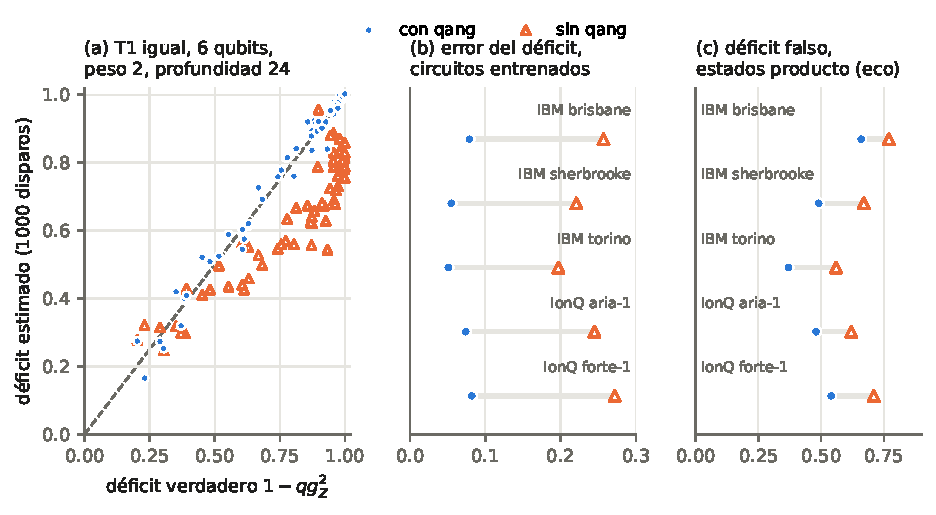
\includegraphics[width=\textwidth]{../radius/fig_radius_es.pdf}
\caption{(a) Déficit estimado contra verdadero, T1 igual, 10 circuitos aleatorios de 6 qubits, 1000 disparos.
(b) Error absoluto medio del déficit en 30 circuitos entrenados, cinco modelos de ruido de equipos. (c) Déficit falso
del qubit excitado de un estado producto después de un circuito de eco (verdad: 0).}
\label{fig:main}
\end{figure}

\section{Modelos de ruido de equipos}

Un equipo agrega errores de compuerta, errores de lectura y el tiempo que una compuerta de dos qubits compilada pasa
fuera del sector de peso, donde un decaimiento puede volver a entrar. Usamos el clasificador de peso 1 y cinco qubits de
la Ref.~\cite{monteverde2026qml} compilado a Qiskit (19 compuertas RBS, 38--62 compuertas nativas de dos qubits), en tres
backends simulados de IBM (Aer) y el simulador en la nube de IonQ con los modelos de ruido aria-1 y forte-1, 1000
disparos. Circuitos entrenados: 30 entradas de prueba de iris, déficit verdadero medio 0.37. Circuitos de eco: un estado
de la base excitado, las 15 compuertas entrenadas y su inversa, verdad 0. Cuatro predicciones se registraron antes de
cualquier corrida con ruido (RESEARCH\_NOTES \S100). Los circuitos de IonQ se enviaron con el conjunto de compuertas
estándar de IonQ; como se vio en la Sec.~\ref{sec:angle}, su compilador puede simplificar circuitos que contienen identidades, así
que las filas de eco de IonQ pueden subestimar el ruido (igual muestran un déficit falso de 0.62--0.71).

\begin{table}[h]
\centering\small
\begin{tabular}{lcccc}
\toprule
backend & error del déficit, entrenados & disparos & déficit falso, eco & compuertas de 2 qubits \\
 & con / sin qang & conservados & con / sin qang & entrenados / eco \\
\midrule
IBM brisbane & 0.079 / 0.257 & 0.69 & 0.66 / 0.77 & 62 / 108 \\
IBM sherbrooke & 0.055 / 0.221 & 0.72 & 0.49 / 0.67 & 62 / 108 \\
IBM torino & 0.051 / 0.197 & 0.74 & 0.37 / 0.56 & 62 / 108 \\
IonQ aria-1 & 0.074 / 0.245 & 0.74 & 0.48 / 0.62 & 38 / 60 \\
IonQ forte-1 & 0.082 / 0.272 & 0.70 & 0.54 / 0.71 & 38 / 60 \\
\bottomrule
\end{tabular}
\caption{El déficit de radio en modelos de ruido de equipos (simulados, no hardware).}
\label{tab:dev}
\end{table}

En los circuitos entrenados el déficit filtrado se equivoca en 0.05--0.08, entre 3.2 y 4.0 veces menos que el no
filtrado (Fig.~\ref{fig:main}b); tres predicciones se cumplieron en los cinco backends. La cuarta falló en los cinco:
predijimos que el filtro quitaría más de la mitad del déficit falso de un estado producto, y quitó entre el 15 y el
33\,\% (Fig.~\ref{fig:main}c). El filtro descarta los disparos que salieron del sector, pero los errores que mueven la
excitación dentro del sector lo pasan; aquí afectan al 10--21\,\% de los disparos conservados en el qubit excitado.
Cerca de un polo el déficit los amplifica: una fracción $\varepsilon$ de disparos desplazados se lee como
\begin{equation}
D=4\varepsilon(1-\varepsilon),
\end{equation}
así que un 10\,\% ya se lee como 0.36. Donde el déficit verdadero es grande, los mismos errores lo cambian poco, y por eso
los circuitos entrenados salen bien.

\section{El ángulo en radianes, separado del radio}\label{sec:angle}

El sesgo polar mezcla dirección y longitud, $\qZ=r\cos\theta$, así que la lectura habitual del ángulo,
$\theta=\arccos\qZ$, se corre hacia $\pi/2$ cada vez que el ruido acorta el vector. El radio los separa:
\begin{equation}\label{eq:theta}
\theta=\operatorname{atan2}\!\big(\sqrt{\qX^2+\qY^2},\,\qZ\big)=\arccos(\qZ/r).
\end{equation}
El ruido despolarizante deja la Ec.~\eqref{eq:theta} igual; el desfase achica solo $\qX,\qY$ y la lleva hacia los
polos, mientras que $\arccos\qZ$ es entonces exacto; el amortiguamiento mueve los dos. Comparamos las dos lecturas con
el mismo total de disparos, 3000 por ángulo: con qang, la Ec.~\eqref{eq:theta} con 1000 disparos en cada base X, Y, Z
(la parte ecuatorial con cuadrados insesgados); sin qang, $\arccos\qZ$ con 3000 disparos en Z (RESEARCH\_NOTES \S102,
seis predicciones).

\begin{table}[h]
\centering\small
\begin{tabular}{lcc}
\toprule
ruido (simulación, 31 ángulos) & con qang & sin qang \\
\midrule
despolarizante 0.1 / 0.2 / 0.3 & 0 / 0 / 0 & 0.122 / 0.213 / 0.294 \\
desfase, coherencia 0.9 / 0.8 / 0.7 & 0.035 / 0.073 / 0.116 & 0 / 0 / 0 \\
amortiguamiento 0.1 / 0.2 / 0.3 & 0.072 / 0.159 / 0.270 & 0.150 / 0.270 / 0.382 \\
\midrule
modelo de ruido de equipo (11 ángulos, 16 compuertas de 2 qubits) & & \\
IBM brisbane / sherbrooke / torino & 0.053 / 0.029 / 0.041 & 0.267 / 0.207 / 0.374 \\
IonQ aria-1 / forte-1, compuertas nativas & 0.028 / 0.026 & 0.249 / 0.226 \\
\bottomrule
\end{tabular}
\caption{Error absoluto medio del ángulo polar (rad). Simulación: valores exactos; modelos de ruido de equipos: 3000
disparos por ángulo.}
\label{tab:theta}
\end{table}

Con ruido despolarizante la Ec.~\eqref{eq:theta} es exacta, mientras que $\arccos\qZ$ se equivoca hasta 0.70 rad cerca
de los polos; con disparos su error cuadrático medio es 5.8 veces menor con $p=0.2$. Con desfase pierde, como estaba
previsto, y sin ruido las tres bases cuestan un factor 1.6. Con amortiguamiento se equivoca entre un 29 y un 52\,\%
menos. En los modelos de ruido de IBM el vector se achica casi de manera uniforme y la Ec.~\eqref{eq:theta} es entre 5
y 9 veces más precisa. En el simulador de IonQ la primera corrida falló: el compilador de IonQ eliminó el bloque de
ruido (pares de CX que se cancelan), así que el vector no se achicó y ganaron los disparos extra en Z. Un estudio
posterior con sus propias predicciones (\S103) lo confirmó: con el conjunto de compuertas estándar de IonQ el bloque no
cambió nada, y enviado como 16 compuertas nativas MS, que IonQ ejecuta tal cual, achicó el vector y la
Ec.~\eqref{eq:theta} fue entre 8.7 y 9.0 veces más precisa. La regla es simple: si el radio medido es casi 1, conviene
$\arccos\qZ$ con todos los disparos en Z; si está claramente por debajo de 1 y el ruido no es solo desfase, conviene la
Ec.~\eqref{eq:theta}. Los circuitos que contienen identidades, como los de eco de arriba, requieren en IonQ el conjunto
de compuertas nativo.

\section{Discusión}

El radio mide entrelazamiento solo si el registro es puro. La conservación del peso y el filtro qg lo garantizan
exactamente bajo un modelo de ruido, T1 igual, y lo hacen con los disparos en la base Z de la lectura, con un costo en
disparos conocido de antemano. Con el ruido de un equipo, el radio filtrado sigue siendo una buena estimación de un
déficit grande, pero no es una prueba confiable de ``no hay entrelazamiento'': los errores dentro del sector, invisibles
para el filtro, hacen que los estados producto parezcan entrelazados. Un déficit chico necesita una calibración, por
ejemplo el circuito de eco usado aquí, o un modelo de error.

\paragraph{Qué es nuevo y qué no.} El radio, su relación con la pureza, el one-tangle y la medida de Meyer--Wallach son
conocidos~\cite{wootters1998,coffman2000,meyer2002,brennen2003}, y también la verificación de
simetrías~\cite{bonetmonroig2018,mcardle2019}. Lo que agregamos es la combinación: que en circuitos de peso fijo el radio
es $|\qZ|$ y se lee con disparos en la base Z, que el filtro lo convierte en una medida de entrelazamiento con T1 igual,
y mediciones de cuánto de eso sobrevive al T1 desigual, al desfase y a los modelos de ruido de equipos, con cada
predicción registrada antes de su corrida, y el ángulo en radianes que el radio libera del ruido.

\paragraph{Limitaciones.} Todo el ruido es simulado, incluidos los modelos de ruido de equipos. Los circuitos son
chicos (4--6 qubits). Los circuitos de eco miden el déficit falso de una sola familia de estados producto. No se afirma
ventaja cuántica.

\section*{Disponibilidad de código y datos}
{\raggedright
Librería \texttt{qang} 0.6.8 (MIT, \texttt{pip install qang}): \texttt{qang.formulation} (\texttt{radius\_profile},
\texttt{radius\_deficit}, \texttt{sphere\_area}, \texttt{meyer\_wallach}, \texttt{weight\_sector\_radius},
\texttt{gate\_radius\_class}, \texttt{algorithm\_radii}, \texttt{direction\_from\_qg}), \texttt{qang.statistics}
(\texttt{qg2\_unbiased}, \texttt{radius2\_estimate}, \texttt{direction\_estimate}). Estudios: \texttt{examples/qg\_radius\_witness\_qg.py} (\S98) y
\texttt{examples/qg\_radius\_hardware\_qg.py} (\S100), \texttt{examples/qg\_direction\_radians\_qg.py} (\S102) y
\texttt{examples/qg\_direction\_ionq\_native\_qg.py} (\S103), con las predicciones en su encabezado y pruebas en
\texttt{tests/}; figura: \texttt{manuscript/radius/make\_figure.py}. Repositorio: \url{https://github.com/Viny2030/qang}.\par}

\section*{Uso de herramientas de IA}
Herramientas de IA generativa (Anthropic Claude Opus 5.5) asistieron con el código, las verificaciones numéricas y la
redacción. El autor propuso la métrica de superficie, planteó las preguntas y revisó y validó todo el material.

\bibliographystyle{unsrtnat}
\bibliography{../refs}
\end{document}
